\textbf{Date:} May 30th 2014\\\textbf{Duration:} 9-14\\\textbf{Group
members:} Henrik, Jakob, Jesper

\subsection{Goals for today:}

We will continue working on the line follower, while some of the group
will start building the mechanism.

We got a P controller for the line follower to work so that it can
follow a line. However the vehicle gets confused when it meets a cross
section. We'll need a way to handle these sections on the track, so
we're gonna implement behavior control.\\We'll have a default behavior
that simply drives forward using the line follower. When the light
sensor picks up lower light values, it'll be overruled by a
turning/navigation behavior. When a solar panel is detected, another
panel checking/manipulating behavior will take over.

We have the first build of the mechanism ready, it just needs to be
added to the vehicle. It's quite large and and will allow for some
inaccuracy of the line following
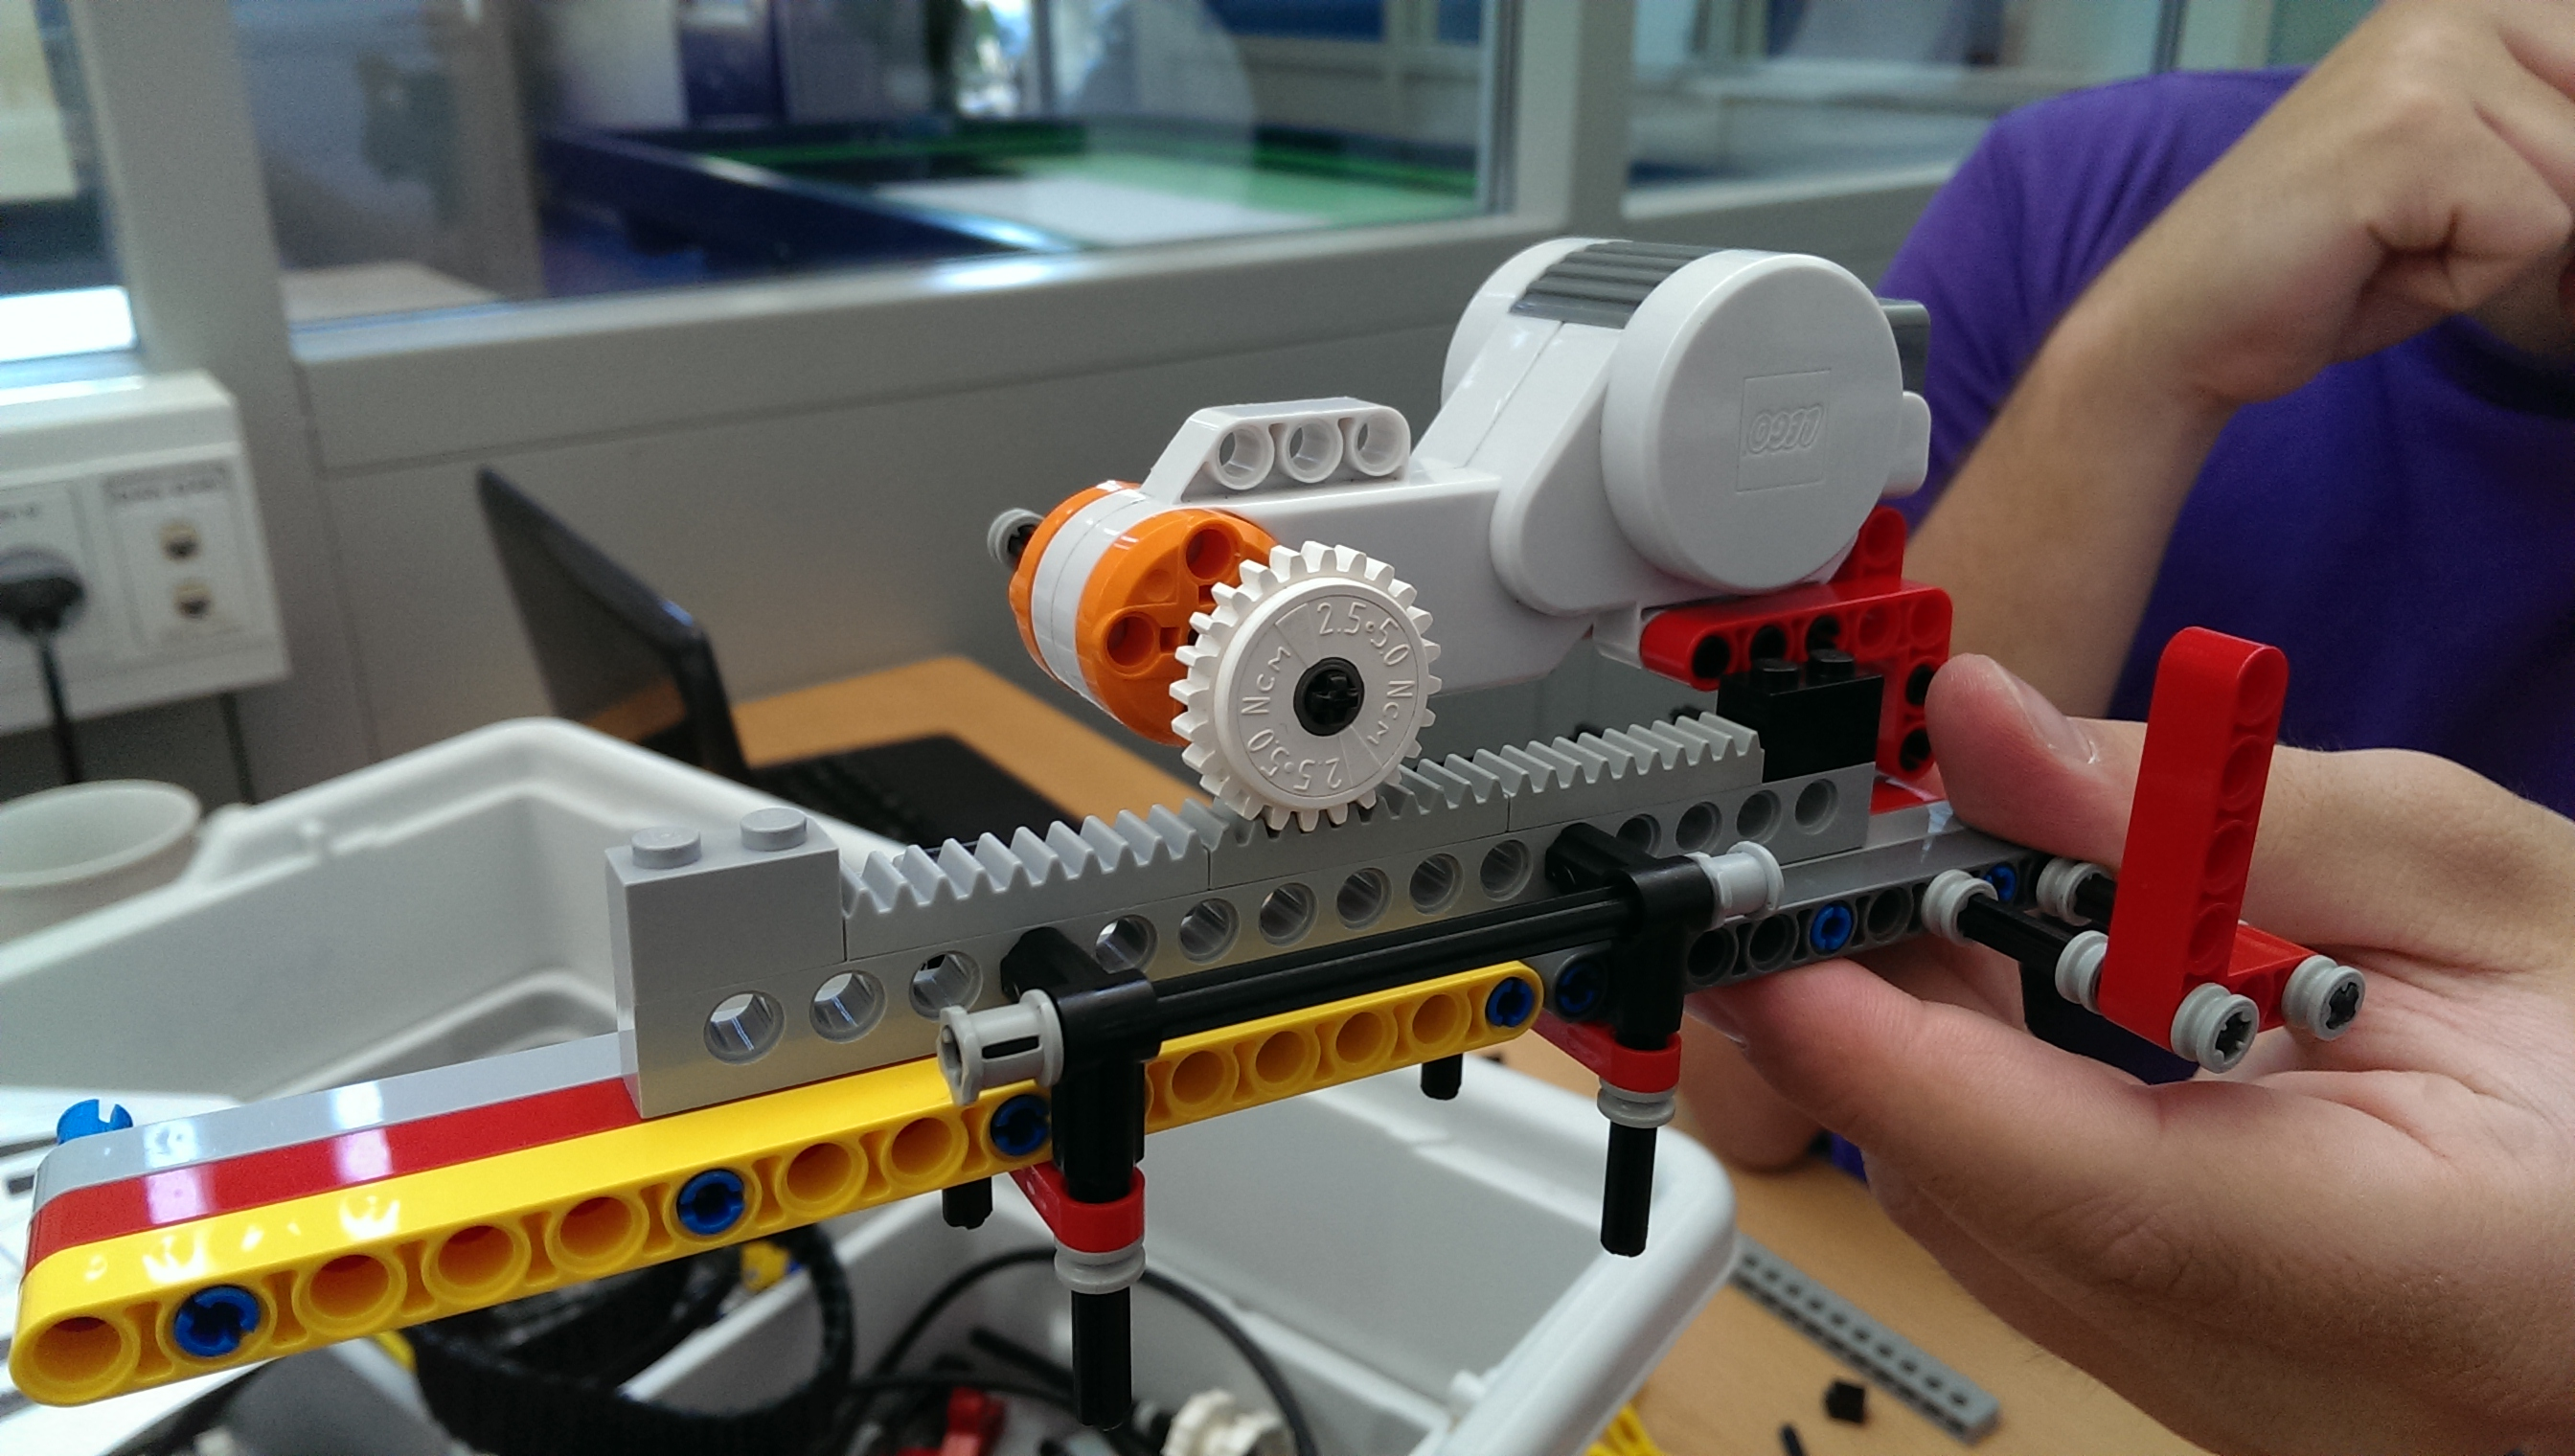
\includegraphics[scale=0.5]{../experiments/images/2014-05-30 12.18.02.jpg}
It uses the motor to drive the cog, making the solar panel slot move
back and forth, allowing us to lock a solar panel in the side of the
vehicle. We need to rebuild the vehicle in order to sport this large
mechanism, and once this is done we'll be able to test the solar panel
manipulation capabilities.

Currently, our proportional controls have a factor Kp = 1.0, and it's
able to follow a line quite
well.\\https://www.youtube.com/watch?v=PJHLTqwCBCI

We have no need for integral or differential control as there are no
sharp or difficult turns on the track. We use the tacho counter turns
from last meeting to do 90 degree turns, as this is a very reliable way
of handling single turns, and after a turn we'll use the line follower
to navigate again, thus finding our way back onto the line. This is a
very promising way of following lines, and as seen in the video it works
very well until we hit the gray areas with solar panels. We've discussed
using a color sensor instead of the light sensor, which will help us
overcome the obstacle that is color recognition at variable light
levels, which caused us trouble previously.

\subsection{Conclusion}

We have an early version of the mechanism built, and a new vehicle is
being built around it. Our old vehicle is able to follow a line and turn
quite well, which we'll need to migrate into the new model.
